% !TeX root = tlk16jun15h.tex


\subsection{Run-Loop}

\frame{\begin{block}{Run-Loop}
%\begin{figure}[hbt]
\begin{center}
\begin{tikzpicture}[scale=0.75, transform shape]
\node[rectangle] (start) at (0,-4em) {};
\node (nc) [myrect] at (0,0) {new\\clauses};
\node (pc) [myrect] at (0,8em) {passive clauses};
\node (ab) [myrect] at (-8em,3.5em) {instantiation};
\node (gs) [myrect] at (-8em,8em) {SMT};
\node (un) [mycircle,colHi,very thick] at (-15em,8em) {un\-satis\-fiable};
\node (se) [myrect] at (-8em,12.5em) {selection};
\node (gc) [myrect] at (0em,16em) {given clause};
\node (ac) [myrect,dashed] at (-14em,16.5em) {active clauses};

\node (sl) [myrect, thick] at (8em,12.5em) {selected literal};
\node (us) [myrect] at (8em,8em) {search for conflicts};
\node (sa) [mycircle, very thick,colLo] at (15em,8em) {satis\-fiable};
\node (su) [myrect] at (8em,3.5em) {substitution};

\node (parse) [myrect,dotted]  at (14em,-2em) {read\\file(s)};

\draw[myarrow, dotted] (parse) to [bend left=20] (nc);
\draw[myarrow] (nc) to (pc);
\draw[myarrow] (nc.west)  to [bend left=10] (ab);
\draw[myarrow] (ab) to (gs);
\draw[myarrow] (gs) to (un);
\draw[myarrow] (gs) to (se);
\draw[myarrow] (pc) to (gc);
\draw[myarrow] (se.north) to [bend left=10] (gc.west);
\draw[myarrow] (us) to (sa);
\draw[myarrow] (us) to (su);
\draw[myarrow] (su) to [bend left=10] (nc.east);
\draw[myarrow] (sl) to (us);
\draw[myarrow] (gc.east) to [bend left=10] (sl.north);
%\draw[myarrow,dashed] (gc.north) to [bend right=15](ac);
\draw[myarrow, dashed] (gc) to [bend right=20] (ac);

\path (nc) edge [myarrow,loop below, dashed] (nc)
 (parse) edge [myarrow, loop above, dotted] (parse)
 (19em,-2em) edge [myarrow,dotted](parse)
;
\end{tikzpicture}
%\caption{Inst-Gen loop with maximal completion}
%\label{fig:inst-gen-maxcomp}
\end{center}
%\end{figure}
\end{block}}

\subsection{Redundancy}
		\frame{
			\begin{block}{Subsumption}
				\vspace{-1em}
%				Subsumed clauses can be removed from a set of first order clauses without affecting satisfiability.
%				Proper instances of clauses affect the satisfiability of the set of ground instances.
				\begin{gather*}
					S = \{C, D, \ldots \}\qquad \exists\theta\ C\theta\subseteq D 
					\tag*{C subsumes D}\\
					 S \text{ satisfiable} 
					 \overset{\text{\colHi\cmark}}\iff (S \setminus D) \text{ satisfiable }
%					   \tag*{Resolution}
					   \\
					   \theta\text{ is proper, }
					S\bot \text{ satisfiable}\ 
%					{\colLo\overset{\text{\colLo\xmark}}{\colLo\Leftarrow \Rightarrow}}
					{\colLo\overset{\text{\xmark}}{\Leftarrow\Rightarrow}}\
					(S \setminus D)\bot \text{ satisfiable } 
%					\tag*{Inst-Gen}
					\\
					\theta\text{ is renaming, }
					S\bot \text{ satisfiable} 
					{\overset{\text{\colHi\cmark}}\iff}
					(S \setminus D)\bot \text{ satisfiable } 
					\end{gather*}
				\end{block}
			
			\begin{Example}[]
				\vspace{-1em}
					\begin{gather*}
\{ 	\mP(x,y), \lnot\mP(\ma,z) \} 
\qquad 
\{ 	\mP(x,y), \lnot\mP(\ma,z), {\colG\mP(\ma,z)} \} 
\\
	\{ \mP(\bot,\bot), \lnot\mP(\ma,\bot) \} 
	\qquad 
	\{ \mP(\bot,\bot), {\lnot\mP(\ma,\bot)},{\colLo\mP(\ma,\bot)} \}
					\end{gather*}
				
				\end{Example}
%							\begin{block}{}
%								Proper instances of clauses affect the satisfiability of the set of ground instances.
%							\end{block}
			}
			
			\subsection{Data structures}
			\frame{
				\begin{block}{needed data structures}
					\begin{enumerate}
						\item representation of clauses, literals and terms
						\item fast retrieval of clauses with a selected literal that is unifiable with the negation selected literal of a given clause
						\item fast retrieval of clauses with a set of literals that is a renamed subset of a given clause
					\end{enumerate}
					
					\end{block}
				}
				
				\subsection{Path indexing}
				\frame{
					% !TeX root = tlk16jun15h.tex
% !TeX encoding = UTF-8
% !TeX spellcheck = en_US

\begin{gather*}
	\{
	\TI{1}\mP(\mf(x,x)),
	\TI{2}\mP(\mg(\ma,x)), 
	\TI{3}\mP(\mf(y,z)),
	\TI{4}\mP(\mg(\ma,y)), 
	\TI{5}\mP(\mf(y,x)), 
	\TI{6}\mP(\mg(y,a))
	\}
\end{gather*}
%
\begin{center}
	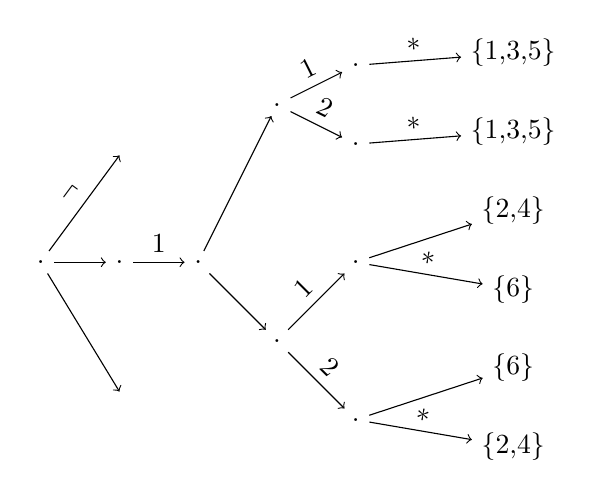
\begin{tikzpicture}[->,sloped,above]
	
	\node (root) at (0,2.5) {.};
	
	\node (h) at (1,2.5) {.};
	
	\node (h1) at (2,2.5) {.};
	
	\node (h1f) at (3,4.5) {.};
	\node (h1g) at (3,1.5) {.};
	
	\node (h1f1) at (4,5) {.};
	\node (h1f2) at (4,4) {.};
	\node (h1g1) at (4,2.5) {.};
	\node (h1g2) at (4,0.5) {.};
	
	\node (h1f1x) at (6,5) {\{1,3,5\}};
	\node (h1f2x) at (6,4) {\{1,3,5\}};
	\node (h1g1a) at (6,3) {\{2,4\}};
	\node (h1g1x) at (6,2) {\{6\}};
	\node (h1g2a) at (6,1) {\{6\}};
	\node (h1g2x) at (6,0) {\{2,4\}};
	
	\path (root) edge node {$\mP$} (h)
	(h) edge node {$1$} (h1)
	
	(h1)
	edge node {$\mf$} (h1f)
	edge node {$\mg$} (h1g)
	
	(h1f)
	edge node {$1$} (h1f1)
	edge node {$2$} (h1f2)
	
	(h1g)
	edge node {$1$} (h1g1)
	edge node {$2$} (h1g2)
	
	(h1f1)
	% edge node {$\ma$} (h1f1a)
	edge node {$*$} (h1f1x)
	
	(h1f2)
	%		edge node {$\ma$} (h1f2a)
	edge node {$*$} (h1f2x)
	
	
	(h1g1)
	edge node {$\ma$} (h1g1a)
	edge node {$*$} (h1g1x)
	
	(h1g2) 
	edge node {$\ma$} (h1g2a)
	edge node {$*$} (h1g2x)
	
	(root)
	edge node {$\lnot$} (1,4)
	edge node {$\mQ$} (1,1)
	;
	\end{tikzpicture}
\end{center}
$\lnot\mP(\mg(\mb,z)) \mapsto \{ \mP.1.\mg.1.{\mb}, \mP.1.\mg.2.{*} \} \mapsto \{6\} \cap \{2,4,6\}$}
				
				\subsection{Discrimination trees}
				\frame{
					% !TeX root = ../m3Handout.tex
% !TeX encoding = UTF-8
% !TeX spellcheck = en_US

\begin{block}{Insert}
	\def\TRIEWIDTH{4cm}
	\def\TEXTWIDTH{\textwidth-\TRIEWIDTH-2em}
	\begin{minipage}{\TEXTWIDTH}
		$
\TI{\ell_1}\mP(\mf(x,y)), 
\TI{\ell_2}\mP(\mf(x,\mh(\ma))),
\TI{\ell_3}\mP(\mf(\mh(\ma),\ma))
$
		\begin{align*}
			t_1 &\Rightarrow \mh.\mf.{*}.{*}\\
			t_2 &\Rightarrow \mh.\mf.{*}.\mh.\ma \\
			t_3 &\Rightarrow \mh.\mf.\mh.\ma.\ma
			\end{align*}
	\end{minipage}
	\begin{minipage}{\TRIEWIDTH}
		\def\pyL{-0.3}
		\def\pxL{-0.0}
		\begin{tikzpicture}[->,dotted]
		\renewcommand{\PAUSE}{\pause}
		\ORIGIN

\def\pyL{-0.2}
\def\pxL{0.05}

\PAUSE

\node (root) at (2.5,5) {.};
\node (h) at (2.5,4) {.};
\path (root) edge node {$\mh$} (h);

\PAUSE
\node (h1) at (2.5,3) {.};
\path (h) edge node {$1$} (h1);

\PAUSE
\node (h1f) at (1.5,2) {.};
\path (h1) edge node {$\mf$} (h1f);

\PAUSE
\node (h1f1) at (0.5,1) {.};
\path (h1f) edge node {$1$} (h1f1);

\PAUSE
\node (h1f1x) at (0,0) {.};
\path (h1f1) edge node {$*$} (h1f1x);
\node (12) at (\pxL,\pyL) {\scriptsize$t_1,t_2$};

\PAUSE
\node (h1f1a) at (1,0) {.};
\path (h1f1) edge node {$\ma$} (h1f1a);
\node (3) at (\pxL+1,\pyL) {\scriptsize$t_3$};

\PAUSE
\node (h1f2) at (2.5,1) {.};
\path (h1f) edge node {$2$} (h1f2);

\PAUSE
\node (h1f2x) at (2,0) {.};
\path (h1f2) edge node {$*$} (h1f2x);
\node (1) at (\pxL+2,\pyL) {\scriptsize$t_1$};

\PAUSE
\node (h1f2a) at (3,0) {.};
\path (h1f2) edge node {$\ma$} (h1f2a);
\node (23) at (\pxL+3,\pyL) {\scriptsize$t_2,t_3$};


\node (lu) at (0,-0.5) {} ;
		\node (lu) at (-3,-5.5) {} ;
		\end{tikzpicture}
	\end{minipage}
	%
\end{block}
					
					\begin{block}{Implementation}
						\vspace{-1em}
%						The literal index is implemented as mapping from yices literals to clauses.
						
						\begin{align*}
							\texttt{ Clause}&\mapsto\mathtt{(Int,\ Set\ of\ term\_t)}\\
						\texttt{ term\_t}&\mapsto \mathtt{Set\ of\ Int}\\
							\texttt{ Int}&\mapsto \mathtt{Clause}
						\end{align*}
						
						\end{block}
					}